\part{Experiment 1: Data analysis system}
\section{3nd Phase: Analyzer system implementation}
Total implementation link for Experiment 1 : \\
\url{https://github.com/Sprea22/Data_Analyzer_Python}

During this part the main purpose is to analyse the whole dataset in order to find some kind of useful informations later on. \\
The Python system that we are going to implement is mainly used for a generic analysis of the data under from different point of views.\\
The output of this phase will basically be for each single data input:
\begin{itemize}
\item Total graphic of the input data from 2005 to 2016.
\item Comparison of the graphics for each single year of the input data from 2005 to 2016.
\item Correlation matrix between different months of the same input.
\item Correlation matrix between different years of the same input.
\end{itemize}


It's important to remind that this phase can be implemented in different ways and with different programming language, in this case the programming language choosen is Python, so be sure to have installed all the necessary for compile and execute Python code on your platform.\\
(PYTHON REQUIREMENTS)\\
During this experiment we are going to implement a system that is basically divided in two subsystems, that are:
\begin{itemize}
\item Single Input Analyzer (SIA): Used for analyze a single data input.
\item Multiple Inputs Analyzer (TIA): Used for analyze multiple data inputs.
\end{itemize}
\newpage
\subsection{Imported libraries}

During the implementation of both the analysis systems we will need the following Python libraries. \\

The "pandas" library will be very useful for read the data from CSV dataset and setup the plot abut it.
\begin{lstlisting}
import pandas as pd
\end{lstlisting}

The "numpy" library it's used for mathematic purpose, such as calculating the correlation coefficent between two series.
\begin{lstlisting}
import numpy as np
\end{lstlisting}
 
The "pyplot" library it's used for basic graphic displaying and customization, easy to use but very efficent.
\begin{lstlisting}
import matplotlib.pyplot as pyplot
\end{lstlisting}

Also the library "sys" would be very useful for test and execute the program, mainly because it allows to input directly from terminal.
\begin{lstlisting}
import sys
\end{lstlisting}

\newpage
\subsection{Single Input Analyzer}
\begin{itemize}
\item SIA part I: Generate and display araphic about current input with total data from 2005 to 2016
\item SIA part II: Generate and display a graphic about current input for each year from 2005 to 2016
\item SIA part III: Generate and display a graphic that contains the correlation matrix between each single year from 2005 to 2016 of the current input.
\item SIA part IV: Generate and display a graphic that contains the correlation matrix between each single months of the year of the current input.
\end{itemize}
\newpage
\subsubsection{SIA section I: Total graphic for all the years}
\textbf{Goal:}\\
Generate and display the total graphic about current input from 2005 to 2016.

\textbf{Requirements:}\\
- Input dataset: CSV format following the Stand\_N \\
- Data content: 144 values, 1 value for each month from 2005 to 2016

\textbf{Code implementation:}\\
During this section of the code we will use the "pandas" library for read the dataset.
\begin{lstlisting}
series = pd.read_csv("DATASET_DIRECTORY", header=0)
\end{lstlisting}

Then using the "pyplot" library we can setup the plot of the input data.
\begin{lstlisting}
series.plot(color="blue", linewidth=1.5)
\end{lstlisting}


Thera are some settings about the axis x just to display the data in the right format, are easy to change and to costume.
\begin{lstlisting}
years = ["2005","2006","2007","2008","2009","2010",
	"2011","2012","2013","2014","2015","2016"]
x = range(144)
pyplot.xticks(np.arange(min(x), max(x)+1, 12.0), years)
pyplot.title(Total graphic from 2005 to 2016")
\end{lstlisting}

There is the possibility to save the graphic like an image and/or display it.
\begin{lstlisting}
pyplot.savefig("OUTPUT_DIRECTORY", format="jpg")
pyplot.show()
\end{lstlisting}




\begin{minipage}{0.5\textwidth}
\textbf{Results:} \\
With this first part of the code we are able to display and save the basic graphic about the current input from 2005 to 2016, that looks like this example:
\end{minipage} \hfill
\begin{minipage}{0.45\textwidth}
\begin{figure}[H]
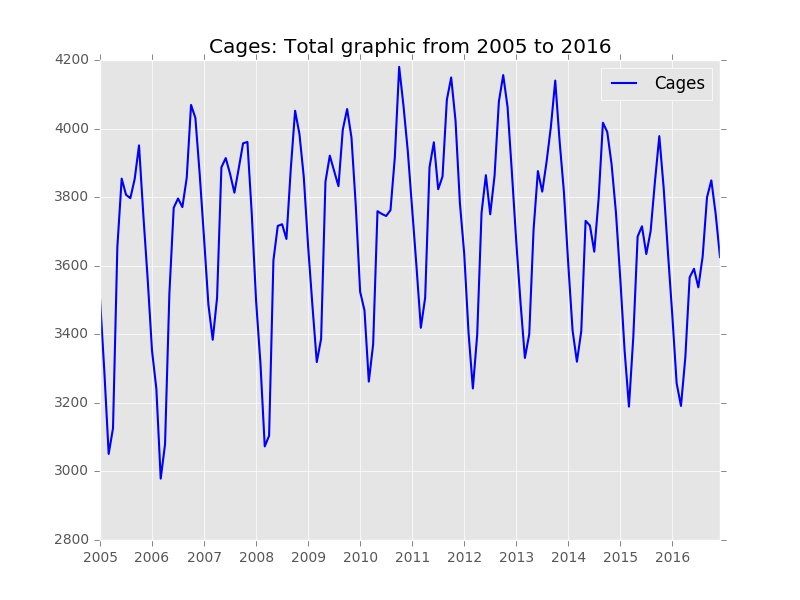
\includegraphics[width=0.9\textwidth]{Files/Cages_Total.jpg}
\caption{Total graphic about current input with total data from 2005 to 2016.}
\end{figure}
\end{minipage}


\newpage
\subsubsection{SIA section II: Single graphics for each year}

\textbf{Goal:}\\
Generate and display graphics about current input for each year from 2005 to 2016

\textbf{Requirements:}\\
- Input dataset: CSV format following the Stand\_M \\
- Data content: 144 values, 1 value for each month from 2005 to 2016

\textbf{Code implementation:}\\
During this section of the code we will use the "pandas" library for read the dataset.
\begin{lstlisting}
series2 = pd.read_csv("DATASET_DIRECTORY", 
	index_col=['Month'], 
	header=0, usecols=[0,1,2,3,4,5,6,7,8,9,10,11,12])
\end{lstlisting}

Then using the "pyplot" library we can setup the plot of the input data.
\begin{lstlisting}
series2.plot()
\end{lstlisting}

Adding the title at the graphic that we are going to display.
\begin{lstlisting}
pyplot.title("Single year's graphic from 2005 to 2016")
\end{lstlisting}

There is the possibility to save the graphic like an image and/or display it.
\begin{lstlisting}
pyplot.savefig("OUTPUT_DIRECTORY", format="jpg")
pyplot.show()
\end{lstlisting}


\begin{minipage}{0.5\textwidth}
\textbf{Results:} \\
With this second part of the code we are able to display and save the graphics about the current input for each single year from 2005 to 2016, that looks like this example:
\end{minipage} \hfill
\begin{minipage}{0.45\textwidth}
\begin{figure}[H]
    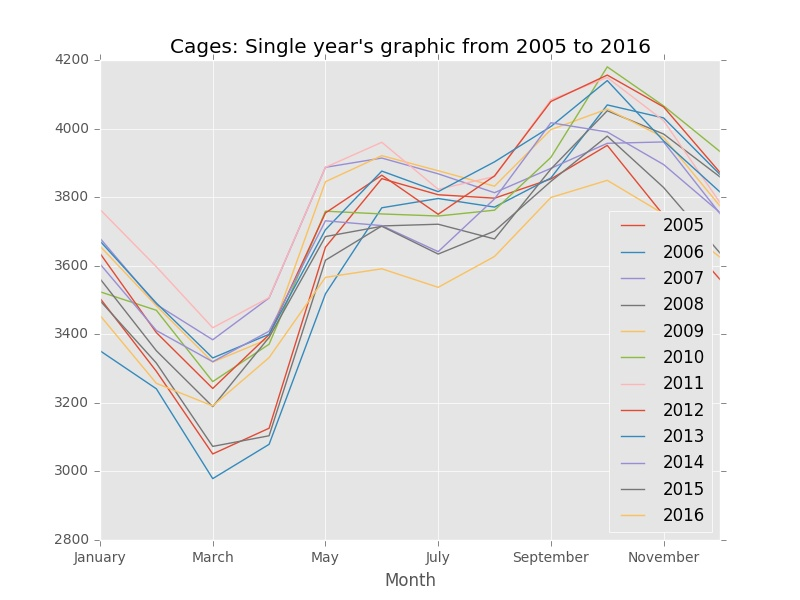
\includegraphics[width=0.9\textwidth]{Files/Cages_Years.jpg}
    \caption{Graphics for each single year of the input data from 2005 to 2016}
\end{figure}
\end{minipage}



\newpage
\subsubsection{SIA section III: Correlation matrix between years}

\textbf{Goal:}\\
Generate and display the correlation matrix about current input between each single year from 2005 to 2016

\textbf{Requirements:}\\
- Input dataset: CSV format following the Stand\_Y \\
- Data content: 144 values, 1 value for each month from 2005 to 2016

\textbf{Code implementation:}\\
During this section of the code we will use the "pandas" library for read the dataset.
\begin{lstlisting}
series3 = pd.read_csv("DATASET_DIRECTORY",
	 header=0, usecols=[1,2,3,4,5,6,7,8,9,10,11,12])
\end{lstlisting}

With the library "numpy" is possible to calculate the correlation coefficents between all the variables in the series just read.
\begin{lstlisting}
test = np.corrcoef(series3.values)
\end{lstlisting}

Setup the figure that will display the correlation matrix using the library "pypot".
\begin{lstlisting}
fig2 = pyplot.figure()
ax = fig2.add_subplot(111)
\end{lstlisting}

Creating the correlation matrix using the already calculated correlation coefficents.
\begin{lstlisting}
cax = ax.matshow(test, interpolation='nearest')
\end{lstlisting}

Settings for display the matrix in the right way, in particular for the values to display on both the axis x and y, in this case every single year from 2005 to 2016
\begin{lstlisting}
years = ["2005","2006","2007","2008","2009","2010",
	"2011","2012","2013","2014","2015","2016"]
x_pos = np.arange(len(years))
y_pos = np.arange(len(years))
pyplot.yticks(y_pos,years)
pyplot.xticks(x_pos,years)
\end{lstlisting}
\newpage
Adding a title to the graphic that we are going to display and also a bar that works like a legend for the colors of the matrix, allowing the reader to better understand the values reported inside the matrix.
\begin{lstlisting}
pyplot.title("Correlation between different years")
pyplot.colorbar(cax)
\end{lstlisting}

There is the possibility to save the correlation matrix like an image and/or display it.
\begin{lstlisting}
pyplot.savefig("OUTPUT_DIRECTORY", format="jpg")
pyplot.show()
\end{lstlisting}

\begin{minipage}{0.5\textwidth}
\textbf{Results:} \\
With this second part of the code we are able to display and save the correlation matrix about current input between each single year from 2005 to 2016, that looks like this example:
\end{minipage} \hfill
\begin{minipage}{0.45\textwidth}
\begin{figure}[H]
    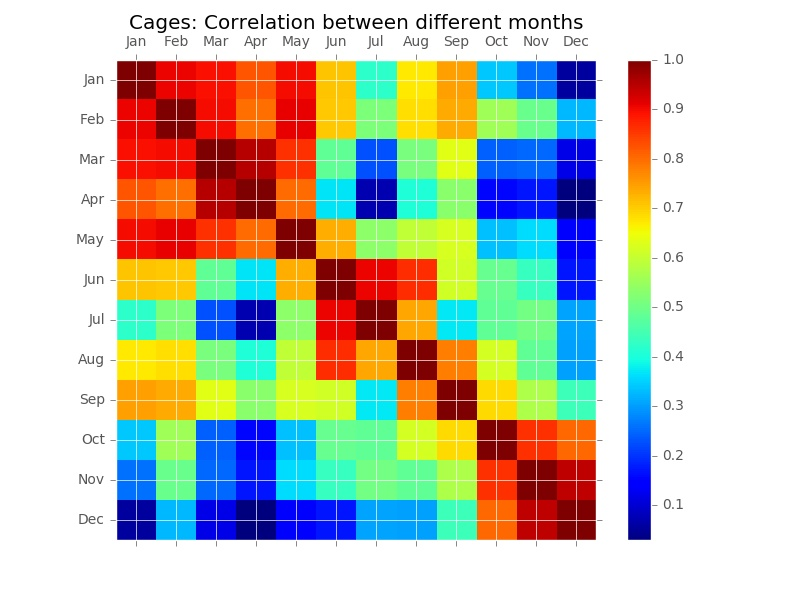
\includegraphics[width=0.9\textwidth]{Files/Cages_Months_Matrix.jpg}
    \caption{Correlation matrix between different months of the same input}
\end{figure}
\end{minipage}



\newpage
\subsubsection{SIA section IV: Correlation matrix between months}

\textbf{Goal:}\\
Correlation matrix about current input between each single month from 2005 to 2016

\textbf{Requirements:}\\
- Input dataset: CSV format following the Stand\_M \\
- Data content: 144 values, 1 value for each month from 2005 to 2016

\textbf{Code implementation:}\\
During this section of the code we will use the "pandas" library for read the dataset.
\begin{lstlisting}
series4 = pd.read_csv("DATASET_DIRECTORY", header=0, 
	usecols=[1,2,3,4,5,6,7,8,9,10,11,12])
\end{lstlisting}

With the library "numpy" is possible to calculate the correlation coefficents between all the variables in the series just read.
\begin{lstlisting}
test = np.corrcoef(series4.values)
\end{lstlisting}

Setup the figure that will display the correlation matrix using the library "pypot".
\begin{lstlisting}
fig2 = pyplot.figure()
ax = fig2.add_subplot(111)
\end{lstlisting}

Creating the correlation matrix using the already calculated correlation coefficents.
\begin{lstlisting}
cax = ax.matshow(test, interpolation='nearest')
\end{lstlisting}

Settings for display the matrix in the right way, in particular for the values to display on both the axis x and y, in this case every single months of the year.
\begin{lstlisting}
months = ["Jan","Feb","Mar","Apr","May","Jun",
	"Jul","Aug","Sep","Oct","Nov","Dec"]
x_pos = np.arange(len(months))
y_pos = np.arange(len(months))
pyplot.yticks(y_pos,months)
pyplot.xticks(x_pos,months)
\end{lstlisting}
\newpage
Adding a title to the graphic that we are going to display and also a bar that works like a legend for the colors of the matrix, allowing the reader to better understand the values reported inside the matrix.
\begin{lstlisting}
pyplot.title("Correlation between different months")
pyplot.colorbar(cax)
\end{lstlisting}

There is the possibility to save the correlation matrix like an image and/or display it.
\begin{lstlisting}
pyplot.savefig("OUTPUT_DIRECTORY", format="jpg")
pyplot.show()
\end{lstlisting}

\begin{minipage}{0.5\textwidth}
\textbf{Results:} \\
With this second part of the code we are able to display and save the correlation matrix about current input between each single month from 2005 to 2016, that looks like this example:
\end{minipage} \hfill
\begin{minipage}{0.45\textwidth}
\begin{figure}[H]
    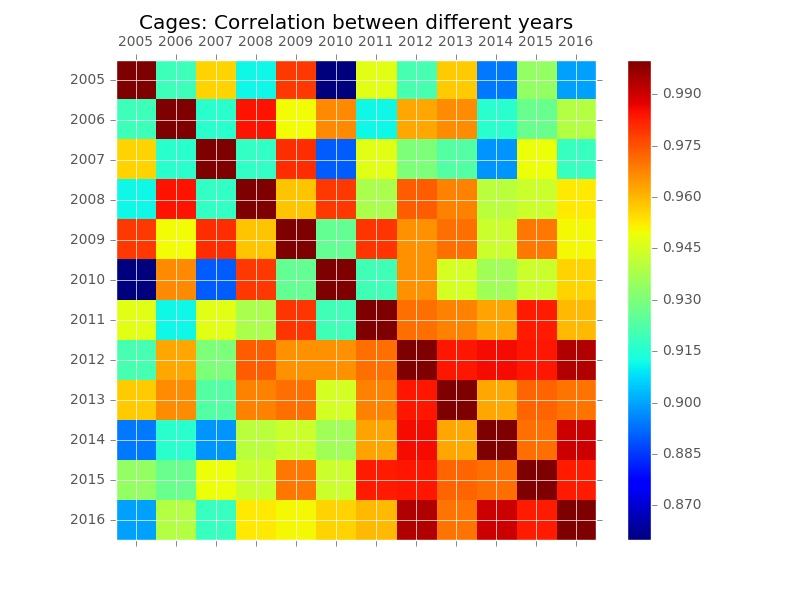
\includegraphics[width=0.9\textwidth]{Files/Cages_Years_Matrix.jpg}
    \caption{Correlation matrix between different years of the same input}
\end{figure}
\end{minipage}



\newpage
\subsection{Multiple Inputs Analyzer}
\textbf{Goal:}\\
This analyzer is mainly used for show the correlation coefficent between the diffent inputs along the total period (from 2005 o 2016), that it will be important to have a general about which kind of relation there is between different inputs and how much strong it is.

\textbf{Requirements:}\\
- Input dataset: Total\_Dataset required, structure already reported here:
\hyperref[table: Total_Dataset]{Total Dataset}

\textbf{Code implementation:}\\
First of all, we are going to use the "pandas" library for read the dataset.
\begin{lstlisting}
series3 = pd.read_csv("TOTAL_DATASET_DIRECTORY", 
	index_col=['Input'], header=0)
\end{lstlisting}

Then with the library "numpy" is possible to calculate the correlation coefficents between all the variables just read above.
\begin{lstlisting}
test = np.corrcoef(series3.values)
\end{lstlisting}

Setup the figure that will display the correlation matrix using the library "pyplot".
\begin{lstlisting}
fig2 = pyplot.figure()
ax = fig2.add_subplot(111)
\end{lstlisting}

Creating the correlationg matrix using the already calculated correlation coefficents.
\begin{lstlisting}
cax = ax.matshow(test, interpolation='nearest')
\end{lstlisting}

Settings for display the matrix in the right way, in particular for the values to display on both the axis x and y, in this case every single input.
\begin{lstlisting}
inputs = ["Cages", "Feed", "Number", "Restock",
	"Local", "Withdr", "Biomass", "Price"]
x_pos = np.arange(len(inputs))
y_pos = np.arange(len(inputs))
pyplot.yticks(y_pos,inputs)
pyplot.xticks(x_pos,inputs)
\end{lstlisting}

Adding a title to the graphic that we are going to display and also a ba that works like a legend for the colors of the matrix, allowing the reader to better understand the values reported inside the matrix.
\begin{lstlisting}
pyplot.title("Correlation between different inputs 
		about data from 2005 to 2016")
pyplot.colorbar(cax)
\end{lstlisting}

In the end, using again the library "pyplot", there is the possibility to save the correlation matrix graphic like an image and/or display it.
\begin{lstlisting}
pyplot.savefig("OUTPUT_DIRECTORY")
pyplot.show()
\end{lstlisting}

\textbf{Results:} \\

\begin{figure}[H]
	\centering
    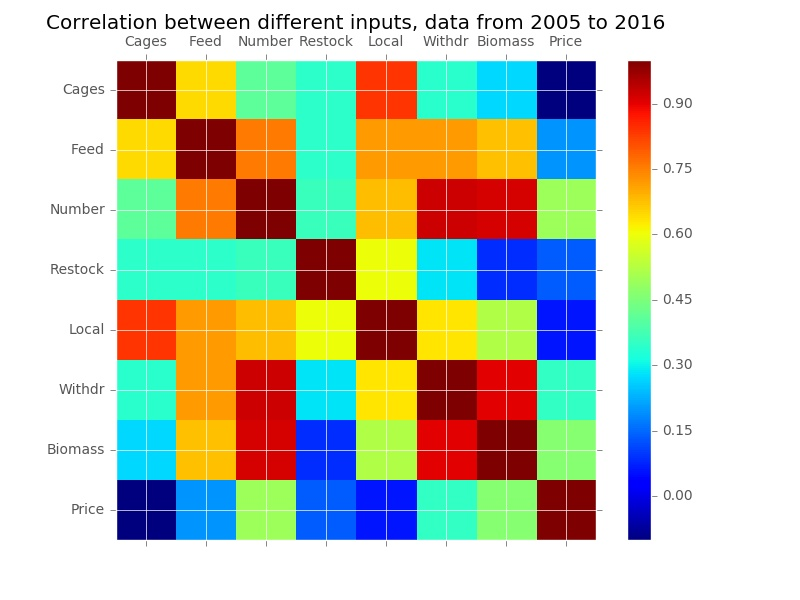
\includegraphics[width=0.75\textwidth]{Files/Total_Dataset_Years_Matrix.jpg}
    \caption{Correlation matrix between different inputs with data from 2005 to 2016}
\end{figure}


\newpage
\section{4th Phase: Data displaying}
\iffalse

\begin{figure}[h]
    \centering
    \begin{subfigure}[t]{0.5\textwidth}
        \centering
        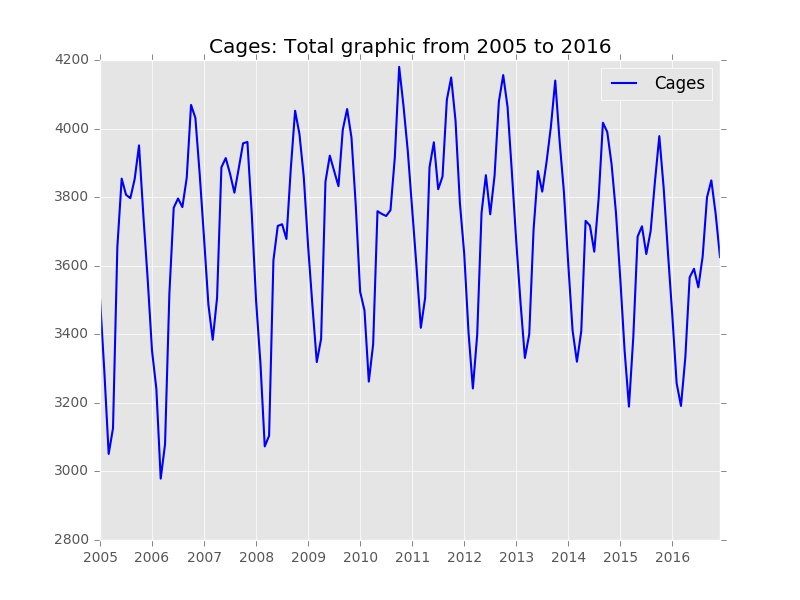
\includegraphics[height=1.2in]{Files/Cages_Total.jpg}
        \caption{Total graphic of the input data from 2005 to 2016}
    \end{subfigure}%
    ~ 
    \begin{subfigure}[t]{0.5\textwidth}
        \centering
        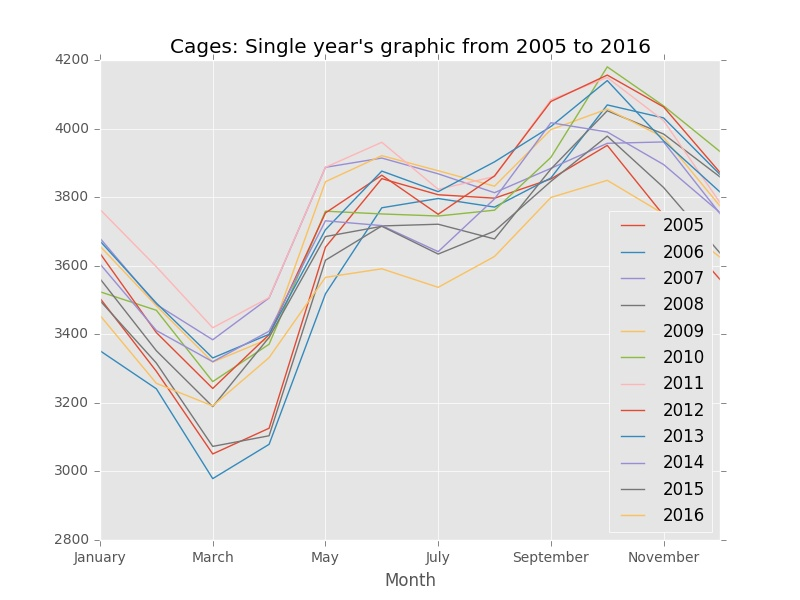
\includegraphics[height=1.2in]{Files/Cages_Years.jpg}
        \caption{Graphics for each single year of the input data from 2005 to 2016}
    \end{subfigure}
    \caption{Data input trends graphics}
\end{figure}

\begin{figure}[h]

    \begin{subfigure}[t]{0.5\textwidth}
        \centering
        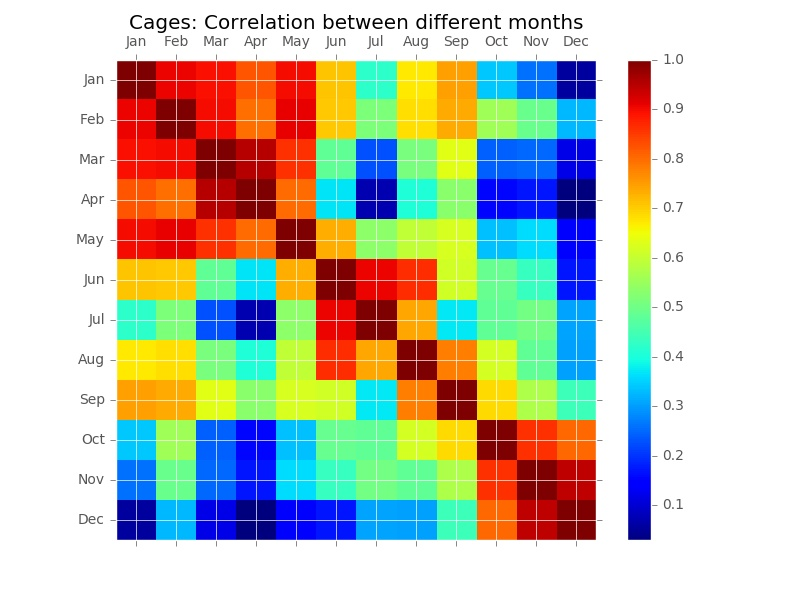
\includegraphics[height=1.2in]{Files/Cages_Months_Matrix.jpg}
        \caption{Correlation matrix between different months of the same input}
    \end{subfigure}%
    ~ 
    \begin{subfigure}[t]{0.5\textwidth}
        \centering
        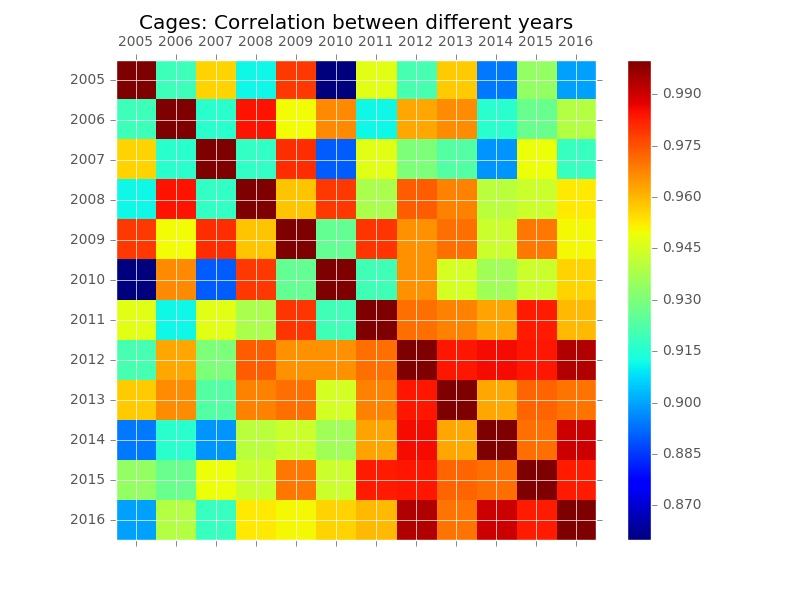
\includegraphics[height=1.2in]{Files/Cages_Years_Matrix.jpg}
        \caption{Correlation matrix between different years of the same input}
    \end{subfigure}
    \caption{Data input correlations matrices}
\end{figure}

\begin{figure}[h]
    \centering
    \begin{subfigure}[t]{0.20\textwidth}
        \centering
        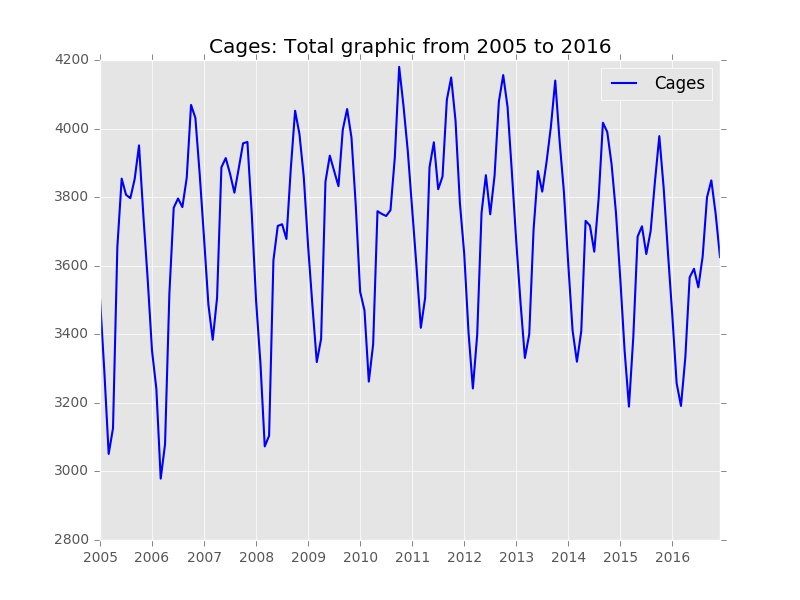
\includegraphics[height=1.2in]{Files/Cages_Total.jpg}

    \end{subfigure}%
    ~ 
    \begin{subfigure}[t]{0.20\textwidth}
        \centering
        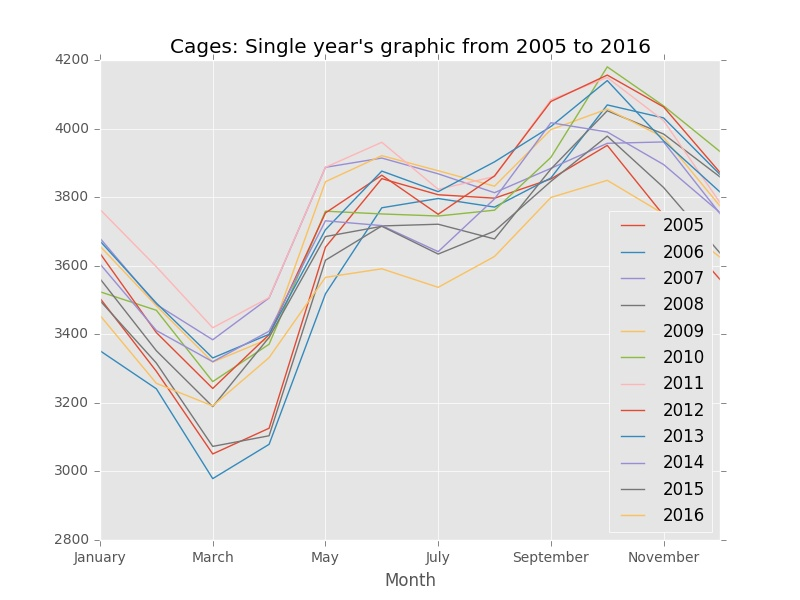
\includegraphics[height=1.2in]{Files/Cages_Years.jpg}

    \end{subfigure}
    ~ 
    \begin{subfigure}[t]{0.20\textwidth}
        \centering
        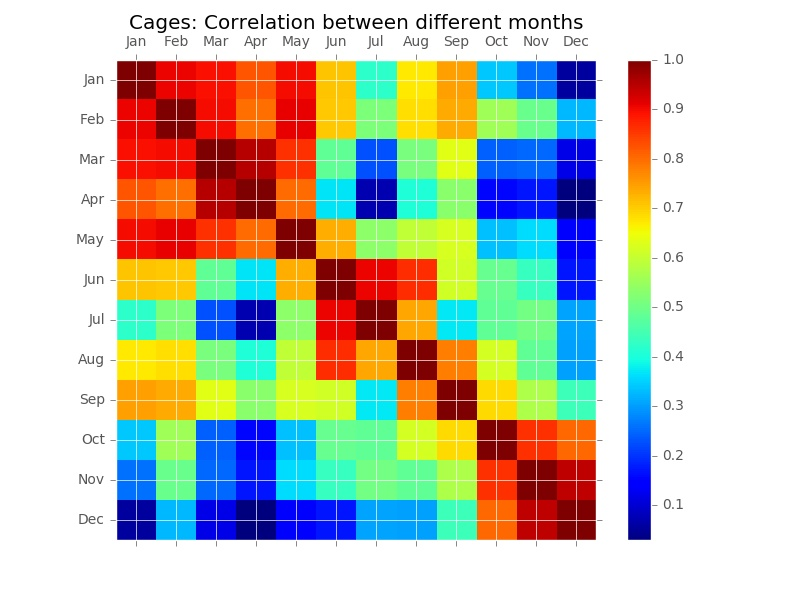
\includegraphics[height=1.2in]{Files/Cages_Months_Matrix.jpg}

    \end{subfigure}%
    ~ 
    \begin{subfigure}[t]{0.20\textwidth}
        \centering
        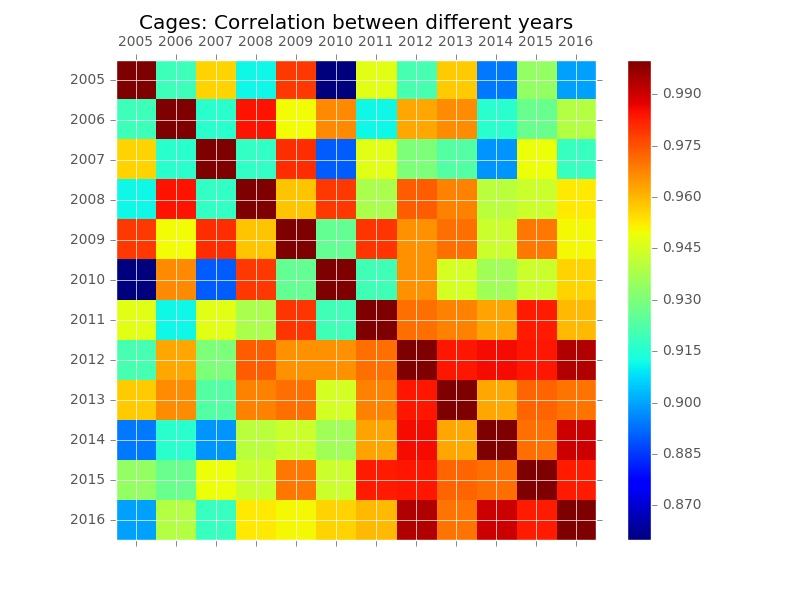
\includegraphics[height=1.2in]{Files/Cages_Years_Matrix.jpg}

    \end{subfigure}

\end{figure}
\fi
